\documentclass[a4paper,14pt]{extreport} % @@ Шрифт 14
\usepackage[utf8]{inputenc}
\usepackage[english,russian]{babel}
\addto{\captionsrussian}{
	\renewcommand{\figurename}{Рисунок}
	\renewcommand{\bibname}{СПИСОК ИСПОЛЬЗОВАННЫХ ИСТОЧНИКОВ}
	\renewcommand{\appendixname}{ПРИЛОЖЕНИЕ}
	\renewcommand{\appendixpagename}{ПРИЛОЖЕНИЕ}
	\renewcommand{\appendixpagename}{ПРИЛОЖЕНИЕ}
}


\usepackage{array}
\usepackage{setspace}
\usepackage[pdftex]{graphicx}
\usepackage{graphicx}
\graphicspath{{img/}}
\usepackage{subcaption}
\usepackage{amsfonts}
\usepackage{amssymb}
\usepackage{amsmath}
\usepackage{url}
\usepackage{listings}
\usepackage[labelsep=endash]{caption}
\usepackage{enumerate}
\usepackage[titletoc]{appendix}
\addto{\captionsrussian}{
	\renewcommand{\appendixname}{ПРИЛОЖЕНИЕ}
	\renewcommand{\appendixpagename}{ПРИЛОЖЕНИЕ}
	\renewcommand{\appendixpagename}{ПРИЛОЖЕНИЕ}
}


\usepackage{algorithm}
\usepackage{algpseudocode}


%\usepackage[nottoc,numbib]{tocbibind} %bibliography in table of contents


\DeclareMathOperator*{\argmaxA}{arg\,max}


\usepackage{titlesec} % decrease chapter heading sizes
    %\titleformat{\chapter}[display]
    %  {\normalfont\large\bfseries\filcenter}{\chaptertitlename\ \thechapter }{0pt}{\Large} %huge 10 Huge
    \titleformat{\section}[block]
	  {\normalfont\large\bfseries}
	  {\thesection}
	  {1em}
	  {}
	\titleformat{\subsection}[block]
	  {\normalfont\large\bfseries}
	  {\thesubsection}
	  {1em}
	  {}
    \titlespacing*{\chapter}
      {0pt}{0pt}{10pt} %10 30 20 default
    \titleformat{\chapter}[block]
     {\normalfont\Large\bfseries\centering}{\thechapter}{1em}{\Large}

    
\makeatletter
\renewcommand{\@biblabel}[1]{#1.} % Заменяем библиографию с квадратных скобок на точку:
\renewcommand{\baselinestretch}{1.25} % @@ Абзацный отступ 1.25
\linespread{1.3} % @@ Межстрочный интервал ~1.5
\makeatother




\usepackage[left=3.0cm,right=1.5cm,top=1cm,bottom=2.0cm,bindingoffset=0cm]{geometry} % @@ Отступы в траницах

\begin{document}

\begin{titlepage}{
		\thispagestyle{empty}\newgeometry{left=2.5cm,right=1.5cm,top=0cm,bottom=0.2cm,bindingoffset=0cm}\setstretch{1}
		\begin{center}
			{\footnotesize
				Министерство образования и науки Российской Федерации\\
				Федеральное государственное автономное образовательное учреждение\\
				высшего профессионального образования\\
			}
									
			<<Уральский федеральный университет\\
			имени первого Президента России Б. Н. Ельцина>>
									
			\vskip+0.5cm
									
			Институт математики и компьютерных наук\\
			Кафедра вычислительной математики
									
			\vskip+60mm
									
			{\bf \LARGE
				Поиск вредоносной активности в DNS трафике \\
			}
									
			\vskip+15mm
		\end{center}
							
		\vfill
		\noindent\begin{parbox}[t]{9cm}{\small
			\vspace{2.0cm}
			Допустить к защите:
									
			\bigskip
			\bigskip
			\bigskip
									
			\hbox to45mm{\hrulefill}
									
			\bigskip
									
			<<\,\hbox to10mm{\hrulefill}\,>>  \hbox to25mm{\hrulefill}  2016 г.
		}
		\end{parbox}
		\begin{parbox}[t]{9cm}{\small  \setstretch{1}
				Выпускная квалификационная работа \\
				на степень бакалавра по направлению\\
				02.03.02
				Фундаментальная информатика \\
				и информационные технологии	 \\
				студента группы МК-420002 \\
				\bigskip
				Меньших Ивана Александровича\\
				Научный руководитель\\
				доцент Солодушкин Святослав Игоревич\\
			}
		\end{parbox}
		\vfill
		\centerline{Екатеринбург}
		\centerline{2016}
		}\restoregeometry
\end{titlepage}


\newpage
\clearpage
\setcounter{page}{\numexpr\value{page}+1}
\chapter*{РЕФЕРАТ}
Выпускная квалификационная работа на степень бакалавра содержит 47 страниц, 7 рисунков, 7 таблиц, 9 источников, 1 приложение.
\newline

Ключевые слова: ВРЕДОНОСНАЯ АКТИВНОСТЬ, DNS ТРАФИК, ДОМЕН, БОТНЕТ, ПРОГРАММНОЕ ОБЕСПЕЧЕНИЕ, ЗАРАЖЕННЫЕ ХОСТЫ, C\&C СЕРВЕР
\newline

Объект исследования - логи DNS сервера.

Цель работы - защита корпоративной сети от вредоносных коммуникаций с C\&C серверами, фильтрация трафика.

Результат работы - программный продукт для нахождения вредоносных доменов в логах DNS сервера а также для выявления паттернов взаимодействия групп зараженных хостов с зараженными доменами.
\addcontentsline{toc}{chapter}{РЕФЕРАТ}  


\renewcommand\contentsname{Содержание}

\tableofcontents
%\addcontentsline{toc}{chapter}{Реферат}  



\chapter{Введение в проблему поиска вредоносной активности}

Важнейшей задачей, стоящей перед системными администраторами, является защита корпоративной сети и пресечение любых вредоносных взаимодействий клиентов сети и сети интернет. Схожая задача стоит перед сервисами, предоставляющими услуги DNS фильтрации. Анализ логов DNS сервера позволяет выделить в общей массе запросов <<подозрительные>> (то есть те, которые соответствуют коммуникации зараженного хоста и, например, управляющего C\&C сервера). 

В реальности, анализ DNS логов проводить крайне трудно, потому что каждый клиент генерирует большое количество запросов. Даже при заходе на сайт пользователь генерирует множество запросов. Как правило, при загрузке страницы происходят обращения на сторонние сервера для загрузки стилей, скриптов, изображений и так далее. Даже когда пользователь ничего не делает, его ПК генерирует запросы. Это могут быть обновления программного обеспечения, синхронизация часов и так далее. Особенно это заметно в новых версиях Windows: операционная система старается <<радовать>> пользователя своей интерактивностью и постоянно запрашивает новости, курсы валют, отправляет различную информацию о его действиях на свои сервера для <<персонализации>> взаимодействия.

В работе будут рассмотрены различные способы анализа DNS трафика, на базе которых можно выделить домены, которые, вероятно, используются для коммуникации между зараженным хостом и ботмастером.

Общая идея заключается в анализе паттернов взаимодействия зараженных клиентов и C\&C серверов. Кроме того, речь будет идти о фильтрации запросов, что является важным аспектом, ведь известно, что <>. Также будут сделаны предположения о структуре паттернов взаимодействия и предложены методы анализа.

\chapter{Формальная постановка задачи}
Для того, чтобы приступить к решению этой проблемы, необходимо формализовать задачу.

{\bfДано:}
		
1. DNS логи ($querylog$). Определим их как множество $Q$. Каждая запись в нем представима в виде вектора признаков $\vec{query}$$\in$$Q$, который обязательно содержит $source\_ip$ (ip адрес клиента, который совершает запрос) и $domain$ (домен, который пользователь желает <<разрешить>>). Кроме того, в нем могут содержаться дополнительные данные, например время, когда был совершен запрос. Подробно структура $\vec{query}$ будет описана далее.
		
2. Белый список доменов ($whitelist$). Будем использовать <<самые частопосещаемые>> домены, для этого воспользуемся списками от Alexa и Quantcast)
		
3. Черный список доменов ($blacklist$). Будем использовать базы компании SkyDNS и прочие источники.
	
{\bfНеобходимо:} 
	
1. Выбрать из $querylog$ подмножество 
запросов $\{\vec{query_1}, \vec{query_2}, \vec{query_3}, \dots\}$, которые были совершены к вредоносным доменам и выделить имена этих доменов. На самом деле наибольший интерес представляют сами доменные имена, так как по ним легко осуществлять блокировку, что и является конечной целью.
	
2. Выделить общие паттерны взаимодействия клиентов и вредоносных доменов, описать внешний вид графа запросов.

\newpage
\section{Структура $\vec{query}, whitelist, blacklist$}
Структура $query$ приводится в таблице~\ref{tab:ql}. В ней описаны типы исходных данных о запросах, которые будут использованы в работе. Стоит обратить внимания, что в <<обычных условиях>> получить их непросто (а именно, если использовать какую либо стандартную реализацию DNS сервера). Процесс сбора этих данных будет описан в главе~\ref{chap:tech}.
\label{sec:strq}
\begin{table}[H]
	\centering
	\caption{Описание структуры $\vec{query}$}\label{tab:ql}
	\begin{tabular}{| c | l |}
		\hline
		Поле     & Описание                                                                 \\ \hline
		$domain$     & Домен, который был запрошен пользователем    \\ \hline 
		$source\_ip$ & IP адрес пользователя                                           \\ \hline
		$rcode$      & Код возврата DNS сервера                                       \\ \hline
		$qtype$      & Код запрашиваемого типа записи                        \\ \hline
		$timestamp$  & Временная метка получения сервером запроса \\ \hline
				
	\end{tabular}
\end{table}


Структура $whitelist$ и $blacklist$ представлена в таблице~\ref{tab:bw}. Это просто списки доменных имен с их категориями. В рамках работы, нас будет интересовать только наличие категории <<вредоносный домен>>. Это единственная априорная информация, которая потребуется для осуществления поиска вредоносных доменов.
\begin{table}[H]
	\centering
	\caption{Описание структуры $whitelist, blacklist$}\label{tab:bw}
	\begin{tabular}{| c | l |}
		\hline
		Поле & Описание                                                                     \\ \hline
		$domain$ & Доменное имя                                                              \\ \hline 
		$cats$   & Список категорий, к которым принадлежит домен \\ \hline
				
	\end{tabular}
\end{table}

\newpage
\section{Словарь}
В таблице~\ref{tab:dict} приведены основные понятия (сокращения), которые будут использованы в данной работе.
\begin{table}[H]
	\centering
	\caption{Основные понятия, используемые в работе}\label{tab:dict}
	\begin{tabular}{|p{3cm}| p{10cm}|}
		\hline
		Термин & Описание                                                                                                                                                                                                                                                                                 \\ \hline
			
		Домен   & Символьное имя, служащее для идентификации областей — единиц административной автономии в сети Интернет — в составе вышестоящей по иерархии такой области. \\ 
		TLD          & Домен верхнего (первого) уровня (например .com, .eu)                                                                                                                                                                                                           \\
		iLD          & Домен i уровня                                                                                                                                                                                                                                                                        \\
		Хост     & Клиентский ПК                                                                                                                                                                                                                                                                        \\
		Ботнет & Сеть из зараженных хостов, управляемая ботмастером через C\&C сервер                                                                                                                                                                      \\
		C\&C         & Управляющий сервер ботнета                                                                                                                                                                                                                                               \\
		whois        & Сервис, позволяющий узнать информацию о регистрации доменного имени, а также о его владельце                                                                                                                       \\
		pDNS         & Техника, позволяющая отслеживать изменения в изменении соответствия доменных имен ip адресам                                                                                                                      \\
		Bind         & Одна из реализаций DNS сервера                                                                                                                                                                                                                                            \\
		\hline
				
	\end{tabular}
\end{table}
	
\chapter{Ботнеты}
\section{Описание}
Ботнет - сеть инфицированных хостов, управляемая извне. Бот, по своей сути, это вредоносное программное обеспечение, которое позволяет злоумышленнику удаленно управлять устройством пользователя.
	
Заражение подобным программным обеспечением может происходить через
уязвимости в используемом ПО (например, через браузер и эксплуатации 0-day exploit, который позволяет исполнить произвольный код за пределами
«песочницы» браузера). Кроме того, заражение может произойти с помощью
«социальной инженерии», где вредоносное ПО маскируется под полезное
содержимое, например, вложение в электронном письме в виде договора, счета или иной важной информации.

Проблема детектирования ботнетов стоит очень остро, так как они растут вместе с интернетом. Например, один из самых больших - ботнет Ponmocup, по данным компании FoxIT, достигал размера 15000000 хостов.
	
Очень важно научиться выявлять ботнеты, а именно, в рамках данной
работы, нас интересуют доменные имена, которые используют C\&C сервера.
Это поможет нам предупредить пользователей, чьи ПК проявляют
«аномальную» активность, схожую с активностью члена ботнета.
	
\section{Топология построения ботнетов}
Можно выделить две основных топологии построения ботнетов, которые подробно рассмотрены в работе $\cite{communication}$.

Топология, изображенная на рис.~\ref{fig:top1} является самой часто встречающейся и простой. Зараженные хосты напрямую обращаются к C\&C серверу. Основная ее уязвимость - централизация. Благодаря этому аспекту, отследить управляющий сервер гораздо проще. Соответственно, и обезвредить такой ботнет легче. Из плюсов стоит отметить быструю коммуникацию, так как отсутствует <<прослойка>> между клиентом и сервером.

\begin{figure}[H]
				
	\begin{subfigure}{0.5\textwidth}
		\includegraphics[width=0.9\linewidth, height=5cm]{star_topology.png}
		\caption{<<Звезда>>}
		\label{fig:top1}
	\end{subfigure}
	\begin{subfigure}{0.5\textwidth}
		\includegraphics[width=0.9\linewidth, height=5cm]{tree_topology.png}
		\caption{<<Дерево>>}
		\label{fig:top2}
	\end{subfigure}
				 
	\caption{Популярные варианты топологии ботнета}
	\label{fig:image2}
\end{figure}
Как расширение данной топологии, можно рассматривать вариант, в котором используется несколько серверов. Это убирает проблему с единой точкой отказа, а также позволяет балансировать нагрузку по географической принадлежности (для общения с хостом используется сервер, который к нему физически ближе). Минус - дополнительные затраты на сервера, а также сложность в синхронизации между серверами.
	
Топология ботнета (рис.~\ref{fig:top2}) встречается реже, но является более устойчивой. Смысл заключается в том, что зараженные хосты общаются с управляющим сервером через <<прокси>>, в качестве которого выступают другие зараженные хосты. Это позволяет скрыть реальный C\&C сервер, что препятствует его обнаружению. Кроме того, ботнет проще будет <<продать>> по частям, продавая контроль над некоторым поддеревом данного графа (а дерево может быть достаточно глубоким).
	
Также встречается топология вида P2P, где хосты соединены между собой и образуют небольшие плотные графы. Это самый устойчивый вариант, но им сложно управлять. В нем просто нет места для C\&C сервера и команды, фактически, передаются какому-либо хосту, который распространяет эту команду всем остальным.

\section{Стратегии уклонения от обнаружения}
Для того, чтобы предотвратить обнаружение управляющий серверов и уничтожение ботнета, ботмастеры используют различные стратегии, препятствующие этому $\cite{communication}$.
\subsection{IP Flux (fast flux)}
Один из вариантов - использовать много ip адресов для одного доменного имени и маленький TTL для A записи в DNS пакете. Данный прием можно усложнить, меняя также ip адреса соответствующий NS серверов.
	
Изначально, данный прием позволял легитимными сайтами балансировать нагрузку между серверами еще на этапе разрешения доменного имени. Этот способ до сих пор используется разными сайтами (например google.com).
	
\subsection{Domain Flux}
\label{ss:dflux}
Другой вариант - использовать много доменных имен, разрешающихся в один ip адрес. Именно этот подход чаще всего используется в настоящее время. Это связано с исчерпанием IPv4 диапазона и, в то же время, доменное имя практически ничего не стоит. Кроме того, владея 2LD доменом, можно легко генерировать множество 3LD доменов (example.com -> *.example.com).
Как правило, для этого используются специальные алгоритмы, которые генерируют домены на основе системного времени. Класс таких доменов называется DGA. Они являются короткоживущими (несколько часов - несколько недель) и используются для одноразовой коммуникации. 



\section{Коммуникация}
Процесс коммуникации, приведенный на рисунке~\ref{fig:comn} можно разделить на несколько шагов.

Описание схемы (рис~\ref{fig:comn}):
	
1. Зараженный хост и управляющий сервер синхронизируют время путем отправки запроса по протоколу NTP к некоторому серверу точного времени. Эта стадия происходит не всегда, если не требуется синхронизации по минутам/секундам. Зачастую, хватает точности до суток.
	
2. Хост и C\&C сервер генерируют доменные имена, основываясь на текущей временной метке.
\begin{figure}[H]
	\centering
	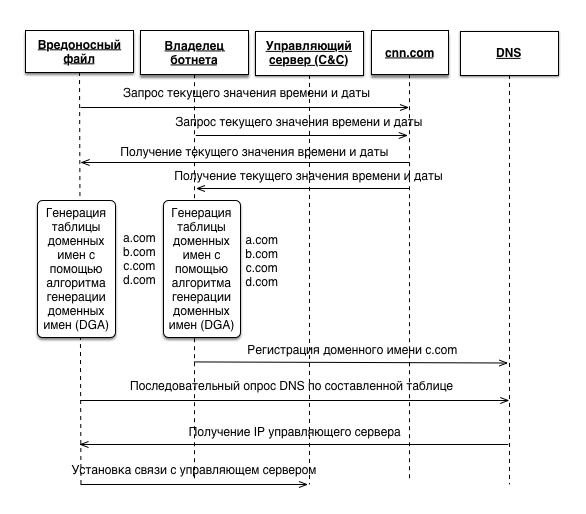
\includegraphics[scale=0.75]{communicate.png}
	\caption{Установка связи между инфицированным хостом и C\&C сервером}
	\label{fig:comn}
\end{figure}

	
3. C\&C сервер регистрирует эти доменные имена.
	
4. Клиент опрашивает сгенерированные доменные имена по списку и пытается получить ip адрес.
	
5. Клиент устанавливает соединение с C\&C сервером и получает необходимые команды/обновления.
	
Таким образом, теперь мы имеем базовое представление о ботнетах, их структуре и поведении.

\chapter{Групповая активность}
\label{chap:groupact}
\section{Основные предположения об активности ботнетов}
Один из подходов поиска ботнетов - отслеживание групповой активности клиент-домен. Основываясь на работе $\cite{groupact}$, сделаем несколько предположений:
	
1. Зараженных хостов в сети фиксированное количество.
	
2. Взаимодействие зараженных хостов и C\&C сервера проявляется периодически.
	
3. Как правило, используется техника domain flux, которая была описана в пункте~\ref{ss:dflux} (используется много доменных имен и мало ip адресов).

4. В случае аномального взаимодействия хостов и домена можно выделить <<периодическое>> взаимодействие узкого круга пользователей с конкретным доменом.
	
Исходя из данных предположений, можно составить алгоритм, который выделит подозрительные коммуникации между группами хостов и доменом.
	
\section{Алгоритм обнаружения групповой активности}
	
Алгоритм поиска групповой активности можно разделить на 3 стадии: сбор информации о запросах пользователей, фильтрация запросов и детектирование подозрительной активности. 
	
Изначально, мы делим все $querylog$ на <<окна>>, в данном случае использовалось окно длины 1 час. Выбрано это число из таких соображений: частая коммуникация не свойственна ботнетам, поэтому не имеет смысл использовать окно меньшего размера. Кроме того, при слишком маленьком окне, высок шанс ложного срабатывания алгоритма, а при слишком большом - слабой чувствительности.
	
Первая функция группирует все пары запросов ($client\_ip$, $domain$) по домену. Подобная агрегация позволяет получить представление о том, кто именно запрашивает конкретный домен.
\begin{algorithmic}
	\Function{SearchInfo}{$querylog$ [by hour]}
	\State $data\gets Dictionary$
	\For{($client\_ip$, $domain$) in $querylog$} 
				
	\State $data[domain]$.add($client$)
	\EndFor
				
	\State \Return $data$
	\EndFunction
\end{algorithmic}

Следующая функция фильтрует полученные данные. Нам необходимо исключить все доменные имена, которые есть в $whitelist$, а также те доменные имена, которые запрашиваются малым количеством пользователей (хорошим вариантом будет значение $threshould$ $\in$ 3, 4, 5, 6, 7)
	

\begin{algorithmic}
	\Function{FilterQueries}{$data$, $whitelist$, $threshould$}
	\For{$domain$ in $data$}
	\If{$domain$ in $whitelist$ OR length(data[domain]) < threshould}
	\State $ip\_list\gets data[domain]$
	\State $data$.remove($domain$)
	\State $data$.pop\_values($ip\_list$)
	\EndIf
					
					
	\EndFor
	\State \Return $data$
	\EndFunction
\end{algorithmic}
	
Последняя функция выполняет предварительную обработку $querylogs$, выбирает доменные имена, к которым в разные временные промежутки обращаются, в основном, одни и те же пользователи, что, в рамках наших начальных предположений, говорит о вредоносности такого домена
\begin{algorithmic}
	\Function{DetectBotnetDomain}{$querylogs$, $sim\_score$}
	\State $data\_arr\gets List$
	\State $botnet\_domains\gets Set$
	\For{$querylog$ in $querylogs$}
	\State $curr\_data\gets SearchInfo(querylog)$
	\State $curr\_data\gets FilterQueries(curr\_data)$
	\State $data\_arr$.append($curr\_data$)
			
	\EndFor
	\For{$data_1$ in $data\_arr$}
	\For{$data_2$ in $data\_arr$}
	\If{$data_1$ $\ne$ $data_2$}
	\For{$domain$ in $data_1$ $\cap$ $data_2$}
	\State $curr\_sim\gets Similarity(data_1[domain], data_2[domain])$
	\If{$curr\_sim$ > $sim\_score$}
	\State $botnet\_domains$.add($domain$)
	\EndIf
	\EndFor
	\EndIf
	\EndFor
	\EndFor
	\State \Return $botnet\_domains$
	\EndFunction
\end{algorithmic}
	
	
Несколько слов о функции $similarity$, она выражает <<схожесть>> между клиентами, которые запрашивают один и тот же домен. В работе $\cite{groupact}$ предлагается для этих целей использовать такую функцию: 
\begin{equation}
	\label{eq:ga-orig}
	similarity(ipList_1, ipList_2) = \frac{1}{2} * (\frac{C}{A} + \frac{C}{B}) (A\ne0, B\ne0)
\end{equation} 
где $$A = |ipList_1|, B = |ipList_2|, C = |ipList_1\cap ipList_2|$$
	
Эксперименты показали, что есть более подходящая функция - расстояние Джаккара: 
\begin{equation}
	\label{eq:ga-jacc}
	similarity(iplist_1, iplist_2) = \frac{|ipList_1\cap ipList_2|}{|ipList_1\cup ipList_2|}
\end{equation} 

Более того, интерпретация расстояния Джаккара интуитивно ясна и, в отличии от функции из работы $\cite{groupact}$, на практике работает ощутимо лучше.
	
\chapter{Графовая модель запросов}
\label{chap:graph}
\section{Описание модели запросов}
В главе~\ref{chap:groupact} была рассмотрена активность групп пользователей относительно доменных имен. В данной главе <<усовершенствуем>> эту идею и перейдем к графовой модели запросов пользователей.
	
Рассмотрим двудольный неориентированный граф ($H\times D$, $E$), где $H$ - множество хостов, $D$ - множество доменных имён, ($h_i$, $d_j$)$\in$ $E$, если пользователь $h_i$ запрашивал домен $d_j$. 
На основе этой модели предлагается вычислять для каждого домена некоторую оценку, которая будет говорить о его вредоносности или же наоборот, о том, что домен <<чист>>. Как мы увидим далее, такая же оценка вычисляется и для хостов, но ее в работе мы использовать не будем.

Идея заключается в том, чтобы передавать через <<соседей>> в графе оценку от доменов к клиентам и обратно. Этот процесс является итерационным.
	
			
Вспомним, что у нас есть $blacklist$ и $whitelist$, в данном разделе будем пользоваться ими для инициализации оценок

\section{Первый вариант ранжирования доменов}
В работе $\cite{graphscore}$ предлагается для оценки использовать процесс случайного блуждания по графу. Использование <<блуждания>> обусловлено тем, что граф получается слишком большой, поэтому они, фактически, вместо точной оценки вычисляют ее приближение. В этой работе, мы будем рассматривать граф, который генерируется на основе 3 часов логов. Так как он помещается в RAM, то мы не будем организовывать случайное блуждание. Мы будем <<честно>> на каждой итерации проходить от каждой вершины ко всем ее соседям и пересчитывать оценку.

Обозначим правила пересчета. На каждой итерации, они симметрично вычисляют оценку для каждой вершины из доли вначале для хостов, потом для доменов по формулам~\ref{eq:dr1-black},~\ref{eq:dr1-white}:
\begin{equation}
	\label{eq:dr1-black}
	black\_score(h_i) = \sum_{d_j: (h_i, d_j)\in E} \frac{black\_score(d_j)}{deg(d_j)}
\end{equation}
\begin{equation}
	\label{eq:dr1-white}
	white\_score(h_i) = \sum_{d_j: (h_i, d_j)\in E} \frac{white\_score(d_j)}{deg(d_j)}
\end{equation}
	
Возникает закономерный вопрос, а зачем нам так много различных оценок, нельзя ли ограничиться просто $black\_score$? Как оказалось, его недостаточно, потому что любой популярный <<чистый>> домен может получить высокую оценку по этому параметру просто из за своей популярности (в графе к нему будет идти много ребер, как от зараженных, так и от <<чистых>> хостов). Именно для этого вводится $white\_score$, который у популярных доменов будет также высоким.
	
Теперь нам нужно <<взвесить>> две полученных оценки, что мы сделаем за счет $union\_score$ по формуле~\ref{eq:dr1-union}:
\begin{equation}
	\label{eq:dr1-union}
	union\_score(d_i) = \frac{black\_score(d_i)}{black\_score(d_i) + white\_score(d_i)}
\end{equation}
По сущетсву, $union\_score$ это отношение <<негативных>> оценок ко всем остальным.

\subsection{Алгоритм вычисления $union\_score$}
\label{alg:us}
Опишем алгоритм пересчета всех оценок на двудольном графе
\begin{algorithmic}
	\Function{CalcScores}{$graph$, $max\_iter$, $whitelist$,  $blacklist$, $init\_weight$}
	\State $black\_score = Dictionary$
	\State $white\_score = Dictionary$
	\State $union\_score = Dictionary$
				
				
	\For{$domain$ in $blacklist$}
	\State $black\_score[domain] = init\_weight$
	\EndFor
				
	\For{$domain$ in $whitelist$}
	\State $white\_score[domain] = init\_weight$
	\EndFor
	\While{$max\_iter > 0$}
	\For{$h_i\in H$}
	\State $black\_score(h_i) = \sum_{d_j: (h_i, d_j)\in E} \frac{black\_score(d_j)}{deg(d_j)}$
	\State $white\_score(h_i) = \sum_{d_j: (h_i, d_j)\in E} \frac{white\_score(d_j)}{deg(d_j)}$
	\EndFor
					
	\For{$d_j\in D$}
	\State $black\_score(d_j) = \sum_{h_i: (h_i, d_j)\in E} \frac{black\_score(h_i)}{deg(h_i)}$
	\State $white\_score(d_j) = \sum_{h_i: (h_i, d_j)\in E} \frac{white\_score(h_i)}{deg(h_i)}$
	\EndFor
	\State $max\_iter\gets max\_iter-1$
	\EndWhile
	\For{$d_i\in D$}
	\State $union\_score(d_i) = \frac{black\_score(d_i)}{black\_score(d_i) + white\_score(d_i)}$
	\EndFor
	\State \Return $union\_score$
	\EndFunction
\end{algorithmic}
	
\section{Второй вариант ранжирования доменов}
Теперь мы используем ту же графовую модель, но с другим правилом пересчета. Это правило упоминается в работе $\cite{rank}$. Само правило выглядит следующим образом (формула~\ref{eq:dr2-rank}):
\begin{equation}
	\label{eq:dr2-rank}
	rank\_score(d_j) = \sum_{h_i: (h_i, d_j)\in E} \frac{rank\_score(h_i)}{deg'(h_i)}
\end{equation}
	
Эта формула схожа с ~\ref{eq:dr1-black}, но есть два серьезных отличия. 

Во-первых, вместо $deg(h_i)$ вычисляем $deg'(h_i)$, который определен не как степень вершины в текущем графе, а как средняя степень текущей вершины по всем графам за некоторый промежуток времени (например за неделю). 

Во-вторых, на этапе инициализации рангов используются оценки разных знаков (положительные для <<чистых>> и отрицательные для <<вредоносных>>), в отличии от алгоритма~\ref{alg:us}, где при инициализации используются только положительные оценки. 

Этот алгоритм очень напоминает алгоритм $PageRank$, но, на самом деле, между ними много отличий, которые приведены в таблице~\ref{tab:pr}.

\begin{table}[H]
	\centering
	\caption{Сравнение $rank\_score$ и $PageRank$}\label{tab:pr}
	\begin{tabular}{|p{7cm}|p{7cm}|}
		
		\hline
		$rank\_score$                                                                                                                                                                       & $PageRank$                                                                                                                                                                  \\ \hline
		Редкое посещение домена <<здоровыми>> клиентами увеличивает шанс того, что домен вредоносный           & Больше связей с хорошими страницами увеличивает шанс того, что страница получит высокий ранг \\ \hline 
		Два типа вершин                                                                                                                                                        & Один тип вершин                                                                                                                                                \\ \hline
		Неориентированный граф                                                                                                                                         & Ориентированный граф                                                                                                                                     \\ \hline
		Фактически, мы имеет разбиение на 3 класса: вредоносные домены, чистые домены и неизвестные домены & Нет разбиения, только ранжирование                                                                                                            \\ \hline
		Вычисляем риск                                                                                                                                                         & Вычисляем популярность                                                                                                                                 \\ \hline
		Очень сильно зависит от начальной инициализации весов                                                                                & Не зависит от начальных весов                                                                                                                      \\ \hline
	\end{tabular}
	\\ 
\end{table}

Это правило пересчёта также похоже на алгоритм $HITS$, если мы превратим наш граф в ориентированный (все рёбра от хостов к доменам) и будем использовать $auth(d_i)$.
	
\subsection{Алгоритм вычисления $rank\_score$}
\begin{algorithmic}
	\Function{CalcRank}{$graph$, $max\_iter$, $whitelist$,  $blacklist$, $init\_weight$, $deg'$}
	\State $rank\_score = Dictionary$
				
	\For{$domain$ in $blacklist$}
	\State $rank\_score[domain] = -init\_weight$
	\EndFor
				
	\For{$domain$ in $whitelist$}
	\State $rank\_score[domain] = init\_weight$
	\EndFor
			
	\While{$max\_iter > 0$}
	\For{$h_i\in H$}
	\State $rank\_score(h_i) = \sum_{d_j: (h_i, d_j)\in E} \frac{rank\_score(d_j)}{deg'(d_j)}$
	\EndFor
					
	\For{$d_j\in D$}
	\State $rank\_score(d_j) = \sum_{h_i: (h_i, d_j)\in E} \frac{rank\_score(h_i)}{deg'(h_i)}$
	\EndFor
	\State $max\_iter\gets max\_iter-1$
	\EndWhile
	\State \Return $rank\_score$
	\EndFunction
\end{algorithmic}

\section{Структура сообществ в графе}
\label{ssec:communitystruct}
Усложним нашу первоначальную модель графа. У нас вновь будет двудольный неориентированный граф ($H\times D$, $E$), где $H$ - множество хостов, $D$ - множество доменных имён. Вся разница в правиле построения рёбер. Ребро ($h_i$, $d_j$, $w_k$) $\in$ $E$, если пользователь $h_i$ запрашивал домен $d_j$ и этот запрос завершился ошибкой (значение поля $rcode$ из DNS-пакета > 0 $\cite{dnsrfc}$, оно присутствует в $querylog$), вес $w_k$ вычисляется как количество запросов, завершившихся ошибкой, от $h_i$ к $d_j$. 

Впервые такой граф фигурировал в работе $\cite{commstruct}$. Пример изображен на рисунке~\ref{fig:subim1}. 

Данный рисунок был отфильтрован от компонент связности, состоящих из двух вершин. Таких компонент в нем более чем 99\% от общего числа компонент связности и для нас они не представляют никакого интереса, так как из за их малого размера мы не может сделать достоверный вывод о их <<природе>>. Кроме того, был взят именно произвольный подграф из за большого размера исходного графа, на котором нельзя визуально увидеть структуру из за обилия ребер.
\\
\begin{figure}[H]
	\center
	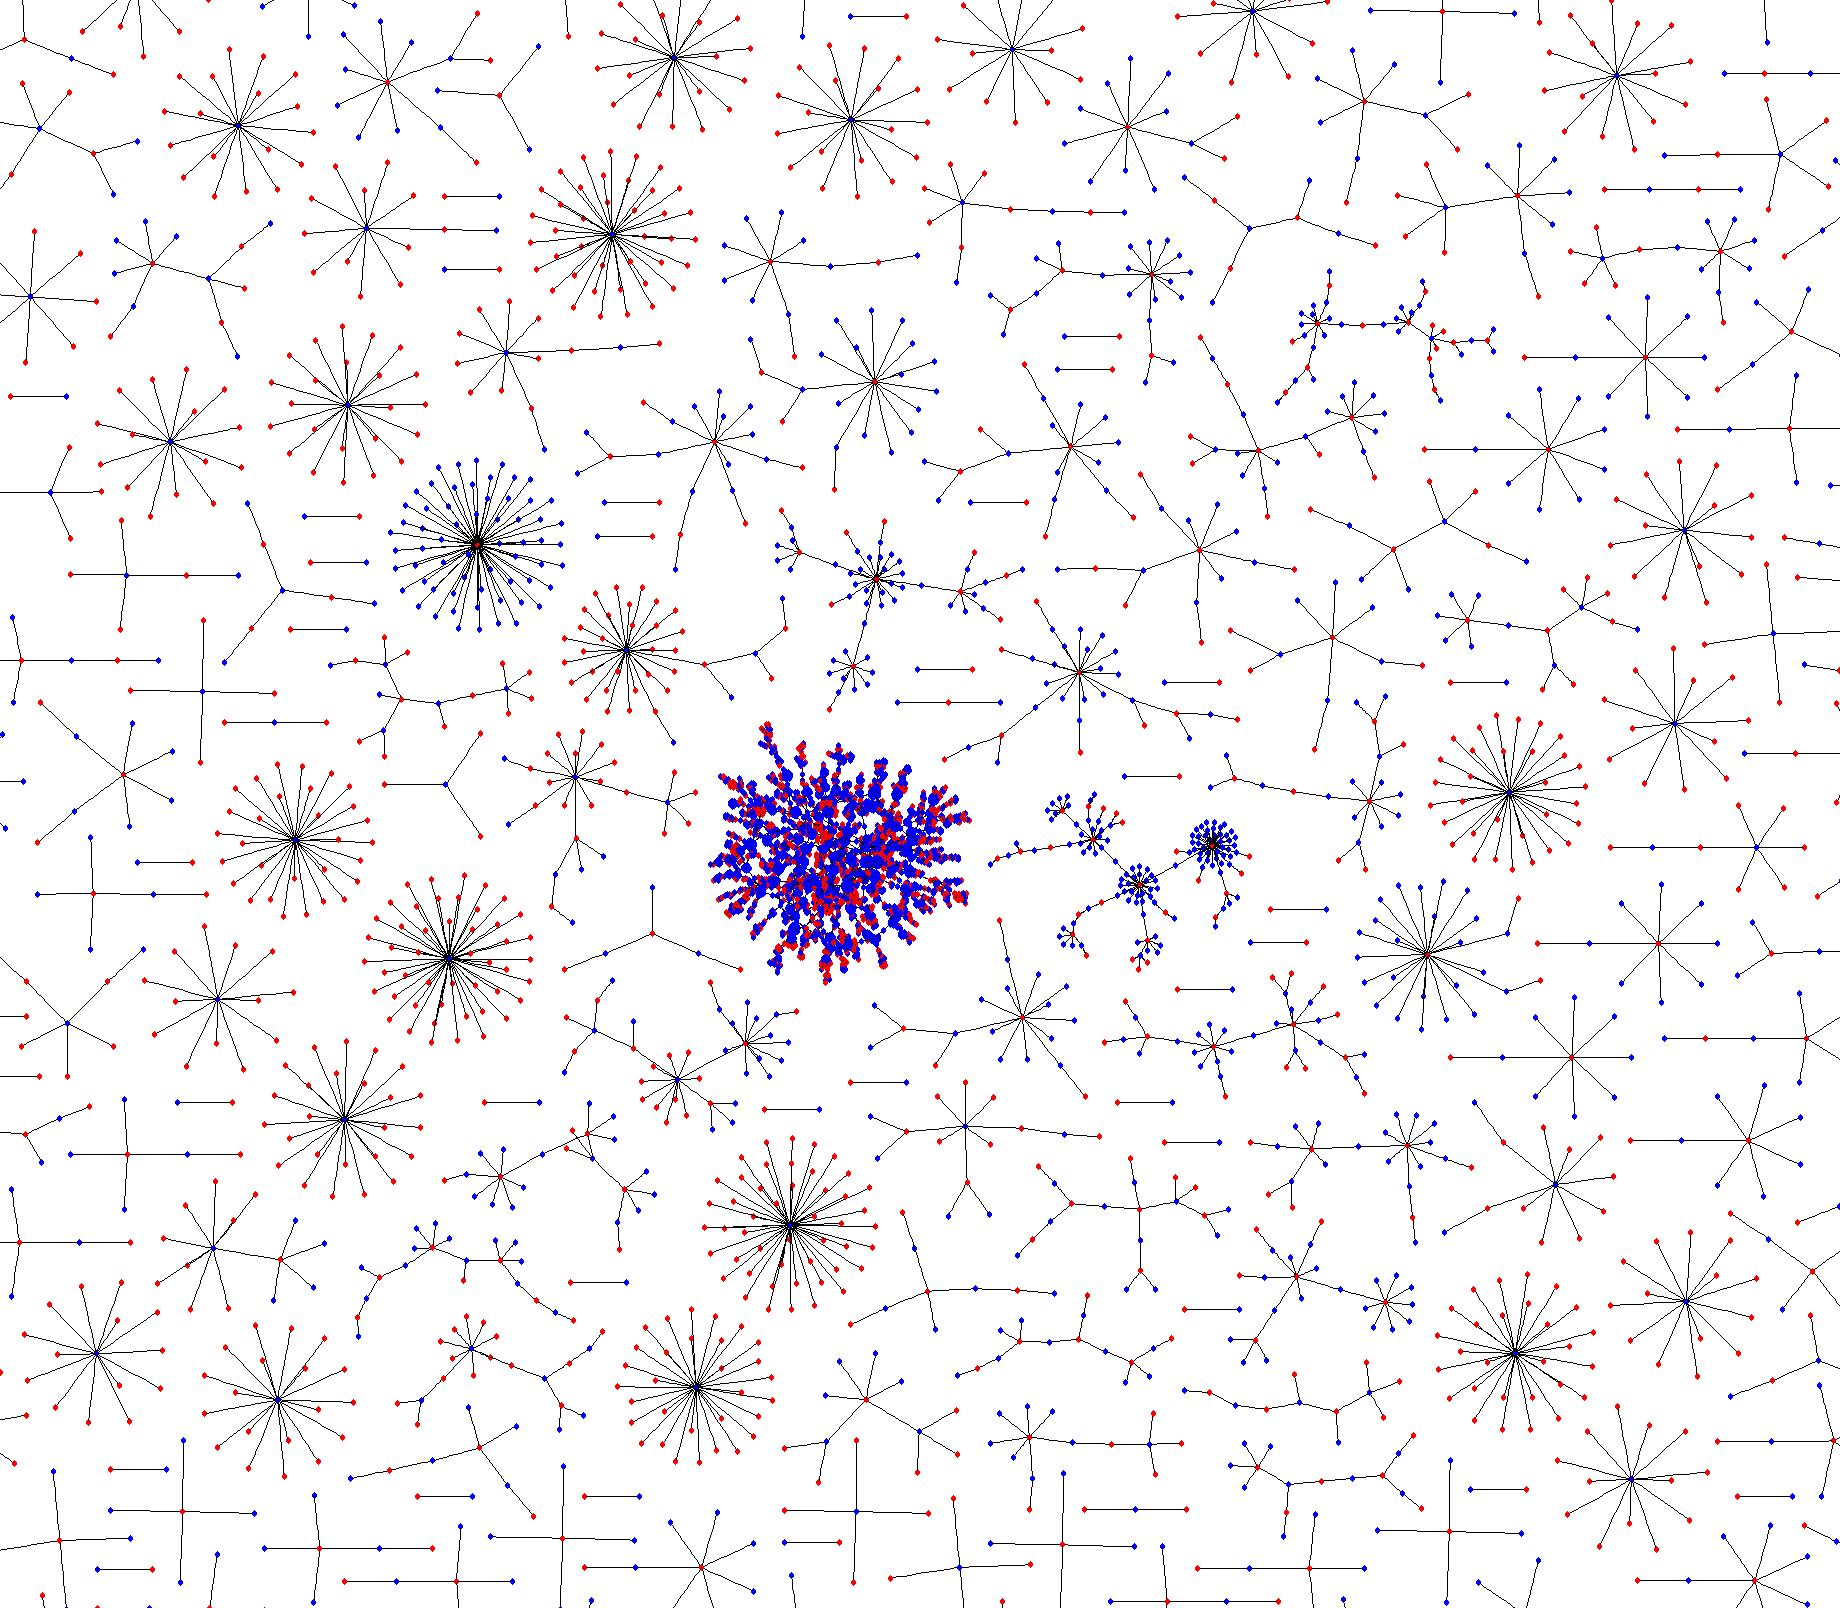
\includegraphics[width=0.9\linewidth]{fail-graph.png}
	\caption{Граф неудачных DNS-запросов (синие - хосты, красные - домены)}
				
	\label{fig:subim1}
\end{figure}
	
	
Из него можно выделить типичные паттерны подграфов.
\begin{enumerate}
	\item <<Звезда>> с доменом в центре. Причины появления:
	      \begin{enumerate}[a)]
	      	\item домен, который существовал ранее, но больше не существует;
	      	\item домен, который является кандидатом на C\&C ботнета;
	      	\item типичная ошибка настройки клиента (например префикс DNS);
	      	\item другое.
	      \end{enumerate}
	\item <<Звезда>> с хостом в центре. Причины появления:
	      \begin{enumerate}[a)]
	      	\item ошибка настройки клиента;
	      	\item перебор возможных доменных имен C\&C сервера;
	      	\item другое.
	      \end{enumerate}
	      	      	      	
	\item Ребро из одного хоста к одному домену. Соответствует запросу редкого домена.
	      	      	      	
	\item Плотный двудольный подграф, соответствует <<сильной>> связи между группами пользователей и группой доменов. Может быть порожден группой клиентов - членов одного и того же ботнета.
	      	      	      	
	\item <<Дерево>>, которое представимо в виде объединения компонент, перечисленных выше
\end{enumerate}
	
\subsection{Алгоритм декомпозиции графа}
Общая идея состоит в построении таких графов и выделении из них плотных подграфов, для которых строится множество признаков, по которому строится классификатор. Опишем основные процедуры этого процесса
	
В первую очередь, нам нужно построить граф ($H \times D$, $E$), при этом выбросим <<мусор>>. Для этого, при построении графа, мы удалим вершины, соответствующие доменам из $whitelist$ (предполагаю, что он содержит популярные домены, на подобие googe.com), также, мы удалим те рёбра, которые имеют $rcode \in (format\_error, serv\_failt, ...)$, т.е. ошибками на стороне DNS сервера, или же при формировании пакета $\cite{dnsrfc}$.
\\
\begin{algorithmic}
	\Function{ConstructGraph}{$querylog$, $whitelist$}
	\State $graph \gets ((\emptyset \times \emptyset$), $\emptyset$)
			
	\For{$query$ in $querylog$}
	\If{$query[rcode] == 0 \vee query[domain] \in whitelist$}
	\State CONTINUE
	\EndIf
	\If{$query[rcode] \in  (format\_error, serv\_failt, ...)$}
	\State CONTINUE
	\EndIf
	\State $graph.add\_node(query[client\_ip])$
	\State $graph.add\_node(query[dname])$
	\State $graph.add\_edge((query[client\_ip], query[dname]))$
					
	\EndFor
	\State \Return $graph$
	\EndFunction
\end{algorithmic}
	
	
Следующий шаг - декомпозиция полученного графа. Процесс будет проходить в два этапа: на первом этапе делается $BFS$, и для полученных компонент связности проводится процесс ко-кластеризации. Достаточно <<плотные>> компоненты мы будем рассматривать на следующем шаге.
\begin{algorithmic}
	\Function{DecomposeGraph}{$graph$, $min\_density$}
	\State $dense\_subgraphs\gets Array()$
	\State $connected\_subgraphs\gets BFS(graph)$
	\For{$graph$ in $connected\_subgraphs$}
	\State $partition \gets coclustering(graph)$
	\For{$g$ in $partition$}
	\If{$density(g)$ > $min\_density$}
	\State $dense\_subgraphs.append(g)$
	\EndIf
	\EndFor
	\EndFor
	\State \Return $dense\_subgraphs$
	\EndFunction
\end{algorithmic}
	
Определим функцию, которая будет говорить о <<плотности>> подграфа таким образом
$$density = \frac{|E|}{|H|*|D|}$$
	
Что касается функции $coclustering$, существуют несколько способов сделать это. В статье $\cite{nmtf}$ предлагается решать задачу 3-факторизации матрицы исходного графа. Опишем формальную постановку задачи 3-факторизации.
	
Пусть $A \in \mathbb{R}_{+}^{m \times n}$ - матрица сопряженности двудольного графа,  $m = |H|, n = |D|$, мы хотим ее разложить на произведение трех матриц $$ U \in \mathbb{R}_{+}^{m \times k}, S \in \mathbb{R}_{+}^{k \times l}, V \in  \mathbb{R}_{+}^{n \times l}$$
$$ A \approx USV^T$$
Оптимизационная задача выглядит так:
$$\min_{U \ge 0, S \ge 0, V \ge 0}{|| A - USV^T||^2}$$
При условиях, что  $U$ и $V$  - ортогональные, $||.||$ - норма Фробениуса.
	
Смысл этого разложения заключается в том, что матрицы $U$ и $V$ отвечают за кластеры по строкам и по столбцам , а матрица $S$ описывает <<тесноту связи>> между парами кластеров (то есть между группой хостов и группой доменов). Описание решения данной задачи можно найти в $\cite{nmtf}$.
	
В результате, мы получаем множество двудольных плотных подграфов, из каждого извлекаем список признаков
	
\begin{enumerate}
	\item Медиана по всем TTL доменов в подграфе. Этот признак может выделить группы короткоживущих доменов, что может свидетельствовать о fast-flux доменах, которые часто используют ботмастера
	\item Отношение количества доменов в графе на количество хостов
	\item Лексические признаки:
	      \begin{enumerate}[a)]
	      		      
	      	\item расстояние между распределение 1-грамм и 2-грамм до равномерного распределения. Для этого есть симметричное расстояние Кульбаха-Лейбнера. Довольно часто доменные имена генерируются с помощью ГСЧ, который, по умолчанию, выдает равномерное распределение;
	      	\item редакторское расстояние между всеми доменами в подграфе. Опять таки, для доменов сгенерированных с помощью ГСЧ будет большим;
	      	\item количество пересекающихся 3-грамм с 3-граммами из $whitelist$ и $blacklist$. Также, к $whitelist$ можно добавить словари популярных языков.
	      \end{enumerate}
\end{enumerate}  

Это достаточно небольшая группа признаков, но уже она даёт результат в распознавании вредоносных подграфов. Больше признаков можно получить, используя $whois$ и $pDNS$.
	
На последнем шаге обучаем классификатор на полученных признаках (для этого, естественно, нужно собрать обучающую выборку, можно опираться на $whitelist$ и $blacklist$). Видно, что этот подход сильно отличается от упоминаемых ранее, так как он базируется не на доменных именах, а на целых подграфах $(H' \times D', E')$. Зато именно этот метод позволяет посмотреть на DNS трафик с более <<высокого>> уровня абстракции и выделить паттерны взаимодействия группы хостов - группы доменов.
	
\chapter{Объединение подходов по оценке доменных имён}
\label{chap:union-all}
В данной работе были рассмотрены несколько подходов детектирования вредоносной активности. В разделе~\ref{ssec:communitystruct} мы получили готовый результат, но он применим только к группам пользователей и доменов. Теперь, нам нужно объединить остальные подходы, которые занимаются оценкой доменов, перечисленные в главах~\ref{chap:groupact} и~\ref{chap:graph}.
	
\section{Описание признаков}
\label{sec:desc-features}
Хорошим вариантом является использование техник машинного обучения, опираясь на выходные данные алгоритмов как на признаки доменов. Опишем те признаки, которые будем использовать. В качестве набора входных данных мы рассматриваем $querylog$ за 3 часа.
\begin{enumerate}
	\item [1--3.] $Similarity$ (формула~\eqref{eq:ga-orig}) для всех пар окон.
	\item [4--6.]$Similarity$ (формула~\eqref{eq:ga-jacc}) для всех пар окон.
	\item [7--9.] Мощность пересечения множеств клиентов по домену (из главы~\ref{chap:groupact}) для всех пар окон.
	\item [10.] $Black\_Score$ (формула~\eqref{eq:dr1-black}) по 3 часам.
	\item [11.] $White\_Score$ (формула~\eqref{eq:dr1-white}) по 3 часам.
	\item [12.] $Union\_Score$ (формула~\eqref{eq:dr1-union}) по 3 часам.
	\item [13.] $Rank\_Score$ (формула~\eqref{eq:dr2-rank}) по 3 часам.
	      	      	      		
\end{enumerate}
\section{Постановка задачи классификации}
Этот набор признаков будем использовать в дальнейшем. Далее сформулируем задачу классификации (на самом деле это задача отбора классификаторов из множества всех обученных классификаторов)
	
{\bf
	Дано:
}

\begin{tabular}{p{6cm} p{7.5cm}}
	$\mathcal{X}=(X_1,\ldots,X_k)$ & входные вектора признаков признаков, $X_i\in\mathbb{R}^n$                \\[0.1cm]
	$\mathcal{Y}=(y_1,\ldots,y_k)$ & вектор правильных ответов (вредоносный ли домен), $y_i\in{0,1}$ \\[0.1cm]
	$(\mathcal{X},\mathcal{Y})$    & обучающая выборка                                                                        \\[0.1cm]
	$(\mathcal{X'},\mathcal{Y'})$  & тестовая выборка                                                                          \\[0.1cm]
	$ROC\_AUC$                     & Функция площади под ROC-кривой                                                    \\[0.1cm]
	$CLF$                          & Множество классификаторов                                                        \\[0.1cm]
	$PARAM$                        & Множество параметров для классификатора                              \\[0.1cm]
			
\end{tabular}
	 
{\bf
	Найти:
} 

Классификатор $clf \in CLF$ такой, что $ROC\_AUC(\mathcal{X'},\mathcal{Y'}) \rightarrow \max$ 
\newline
	
Стоит пояснить, что такое $ROC\_AUC$ и вспомогательные понятия, необходимые для его вычисления. 
	
$ROC\_curve$ - характеристика качества классификатора, зависимость доли верных положительных классификаций от доли ложных положительных классификаций при изменении порога решающего правила. Для построения этой кривой необходимо вычислять $FPR$ и $TPR$ по формулам~\eqref{eq:fpr} и \eqref{eq:tpr}:
	
\begin{equation}
	\label{eq:fpr}
	FPR(clf, (X, Y)) = \frac{\sum_{(x, y) \in (X, Y)}[clf(x)=+1][y=-1]}{\sum_{(x, y) \in (X, Y)}[y=-1]},
\end{equation}
	
\begin{equation}
	\label{eq:tpr}
	TPR(clf, (X, Y)) = \frac{\sum_{(x, y) \in (X, Y)}[clf(x)=+1][y=+1]}{\sum_{(x, y) \in (X, Y)}[y=+1]},
\end{equation}
	
где $clf$ - решающее правило, $X$ - множество векторов, $Y$ множество правильных ответов.
	
$ROC\_curve$ проходит через точки (0, 0), соответствующей максимальному значению порога и (1, 1), соответствующей минимальному значению порога.
$ROC\_AUC$ вычисляется как площадь под кривой $ROC\_curve$.
	
В качестве множества классификаторов возьмём $RandomForest$ и $AdaBoost$, т.к. ансамблевые модели достаточно мощные и <<неприхотливые>> в плане входных данных (не требуют, например, нормализации данных).
	
Для каждого из них будем подбирать основные параметры. В случае с $AdaBoost$ будем подбирать количество деревьев и скорость обучения. В случае же с $RandomForest$ будем выбирать количество деревьев, информационный критерий и максимальное количество признаков, по которым можно производить разделение.
	 
	 
\section{Алгоритм обучения классификатора}
Перечислим шаги, необходимые для получения итогового классификатора
\begin{enumerate}
	\item Весь объем $querylog$ делим на части по 3 часа в каждой, каждая часть будет использоваться как входные данные для итогового алгоритма. Шаги далее будут описаны для работы с одной такой частью.
	      	      	      	
	\item Вычисляем признаки 1 -- 9 из~\ref{sec:desc-features}. Для их вычисления не требуется никакой дополнительной информации
	      	      	      	
	\item Строим двудольный граф $(H \times D, E)$.
	      	      	      	
	\item Берем исходные $blacklist$ и $whitelist$, перемешиваем и делаем 4 независимых разбиения на обучающую и тестовую выборки в соотношении 70/30 
	      (такой подход именуется $KFold CV$).
	      	      	      	
	\item Для каждого такого разбиения $(X\_train, y\_train)$, $(X\_test, y\_test)$
	      \begin{enumerate}[a)]
	      	\item вычисляем признаки 10--13 (используя для начальной инициализации $(X\_train, y\_train)$;
	      	\item для каждой пары $(clf_i, param_i) \in CLF\times PARAM$
	      	      \begin{enumerate}[-]
	      	      	\item обучанем классификатор $clf_i$ с параметрами $param_i$ на множестве $(X\_train, y\_train)$;
	      	      	\item вычисляем $ROC\_AUC(X\_test, y\_test)$.
	      	      \end{enumerate}
	      	      	      	      	      	      	
	      \end{enumerate}
	      	      	      	
	\item Вычисляем
	      \begin{equation}
	      	\label{eq:clf-opt}
	      	clf, param = \argmaxA_{(clf_i, param_i) \in CLF\times PARAM}mean(ROC\_AUC(X\_test, y\_test))
	      \end{equation}
	\item Берем целиком $whitelist$ и $blacklist$ и вычисляем признаки 10 -- 13.
	\item Обучаем классификатор $clf$ с параметрами $param$ на всей выборке.
\end{enumerate}
	
	
Итоговый классификатор мы единожды используем для поиска новых вредоносных доменов на том же графе. После чего процесс повторяется для новой трехчасовой последовательности $querylog$.
	
Фундаментальный принцип, заложенный в процесс обучения классификатора - это кросс-валидация. Далее, я буду понимать под классификатором двойку $(clf, param) \in (CLF, PARAM)$. 
	
Выбирается самый <<стабильный>> классификатор относительно $k$ различных произвольных разбиений обучающей выборки (напомню, что мы разбиваем на 4 части), таким образом получается самый <<качественный>> вариант (метрика $ROC\_AUC$ удобна для сравнения классификаторов между собой). Слово <<стабильный>> следует понимать так: для любого из исходных разбиений выборки, классификатор работает достаточно <<качественно>>
	
Принцип, заложенный в шаги 5 -- 6 называется $GridSearch$. Обучение классификатора - это некоторая задача оптимизации. Тут же мы строим оптимизационную задачу на более высоком уровне. Мы оптимизируем по всем классификаторам, максимизируя <<качество>> классификации. Эта <<метазадача>> (формула~\eqref{eq:clf-opt}) позволяет выбрать наилучший классификатор из представленных.
	

\chapter{Техническая реализация}
\label{chap:tech}
В этой главе речь пойдет непосредственно о реализации алгоритмов, предложенных в данной работе и использовании их в реальной жизни. В качестве источника $querylog$ будем использовать DNS сервера компании SkyDNS. 

\section{Инфраструктура сбора $querylog$}
На рисунке ~\ref{fig:collect-log} ниже изображен процесс сбора логов с серверов.
\begin{figure}[H]
	\center
	\includegraphics[width=1.\linewidth]{dns-comm.png}
	\caption{Сбор логов с DNS-серверов}
				
	\label{fig:collect-log}
\end{figure}
Пользователи DNS серверов обозначены как $host_i$, DNS сервера обозначены как $DNS\_server_j$. Таких серверов около 10 штук. Collector - это сервер, на который собираются $querylog$ и на котором запускаются алгоритмы их обработки. Этот сервер раз в сутки соединяется со всеми DNS серверами и <<выкачивает>> новые $querylog$ (всё это делает обычный скрипт на bash с помощью rsync).

Важно отметить, что в текущей архитектуре DNS сервер состоит из 2 частей: сам DNS сервер (Bind) и прокси, который стоит перед ним и пропускает через себя все запросы пользователей. Это нужно для того, чтобы реализовывать персональную фильтрацию для каждого из пользователей. Для этого в DNS пакет добавляется токен, которому соответствуют конкретные настройки фильтрации. 

Важно, что именно прокси записывает необходимые нам $querylog$ на диск. Эту задачу нельзя переложить на Bind, так как при включении логгирования запросов время его ответа увеличивается нелинейно, в зависимости от количества запросов. Следовательно, при большом количестве запросов, он существенно замедляется, что сказывается на комфорте пользователей, а это неприемлемо. Подтверждение данных слов можно найти в презентации  $\cite{bind}$.

Также, прокси записывает дополнительную информацию (например, profile\_id пользователя и категории, которые присвоены запрашиваемому домену). Всю эту информацию Bind не может логгировать по техническим причинам.

\section{Процесс обработки $querylog$}

Далее начинается процесс обработки $querylog$, который подробно изображён на  рисунке~\ref{fig:full-proc}. Эта схема позволяет увидеть целостную картину, объединяющую подходы, описанные в данной работе.


В синей зоне изображены части $querylog$, которые Сollector собрал с DNS серверов.

В красной зоне происходят общие операции, необходимые для обоих подходов. Вначале происходит группировка $querylog$ на непрерывные трехчасовые блоки по каждому серверу, на каждую такую группу впоследствии будут применены все остальные операции. Далее $querylog$ разбираются (из них извлекаются $client\_ip, dname$ и другие необходимые поля), после чего строятся графы, описанные в главе ~\ref{chap:graph}. 

В желтой зоне происходит процесс обработки, описанный в разделе~\ref{ssec:communitystruct}. В текущий момент, этот процесс не является полностью автоматизированным, так как он требует инфраструктуры для сбора дополнительной информации (признаков), которые требуются классификатору. На текущий момент, из этой зоны мы можем получить лишь плотные подграфы, которые рассматриваются вручную. Мы можем фильтровать эти подграфы по содержанию в них вредоносных доменов, тем самым существенно уменьшив их количество. Для нас такой подграф дает информацию о новых вредоносных доменах, о пользователях, которые находятся в одном ботнете а также раскрывает часть структуры ботнета.

\begin{figure}[H]
	\center
	\includegraphics[width=0.75\linewidth]{clf-schema.png}
	\caption{Процесс обработки и анализа $querylog$}
				
	\label{fig:full-proc}
\end{figure}


В фиолетовой зоне происходит построение классификатора для поиска вредоносных доменов. Данный процесс подробно расписан в главе~\ref{chap:union-all}.

В зеленой зоне содержатся результаты работы всех алгоритмов. В одном случае, это вредоносные подграфы, в другом же - доменные имена. В компании SkyDNS эта информация используется для блокировки доменных имен (на этапе разрешения адреса DNS сервером), что позволяет уберечь пользователя от невольного участия в DDoS атаке. Кроме того, данная информация позволяет уведомлять пользователей о вредоносной активности на их ПК. Кроме того, информация полезна антивирусным компаниям, так как именно они занимаются обнаружением и уничтожением ботнетов (что есть достаточно трудоемкий процесс).
\section{Описание скрипта для поиска вредоносных доменных имен}
Данный скрипт (реализующий подход, описанный в главе~\ref{chap:union-all}) написан на языке python версии 2.7, реализован в виде консольной утилиты, принимающей на вход параметры, описанные в таблице~\ref{tab:keys}.
\begin{table}[H]
	\centering
	\caption{Ключи для запуска скрипта}
	\label{tab:keys}
	\begin{tabular}{|p{3cm}|p{5cm}|p{7cm}|}
		\hline
		Ключ    & Параметр           & Описание                                                                           \\ \hline
		--help      &                            & Показать справку                                                            \\ \hline
		--files     & [filename [filename ... ]] & Список $querylog$ файлов для обработки                             \\ \hline
		--blacklist & filename                   & Список заведомо вредоносных доменов                        \\ \hline
		--whitelist & filename                   & Список заведомо чистых доменов                                  \\ \hline
		--output    & filename                   & Выходной файл с предсказаниями                                  \\ \hline
		--n\_folds  & number                     & Количество разбиений выборки при кроссвалидации \\ \hline
		--n\_iter   & number                     & Количество итераций при просчете рангов доменов  \\ \hline
		--verbose   &                            & Отладочный вывод                                                            \\ \hline
	\end{tabular}
\end{table}

В среднем, полная обработка 3 часов $querylog$ с помощью этого скрипта занимает 30 минут (варьируется в зависимости от количества запросов к DNS серверам в пределах от 10 до 40 минут). Каждый день, алгоритм находит около 5 тысяч новых вредоносных доменов. Исходный код данного скрипта содержится в приложении~\ref{appendix:code}.


\section{Описание скрипта для поиска вредоносных подграфов}
Данный скрипт также реализован на языке python в формате IPython Notebook. У этого формата есть ряд преимуществ, например, быстрое изменение исходного кода, работа в браузере и возможность <<пересчета>> отдельных блоков кода. Настоящий подход достаточно удобен, так как вредоносные подграфы используются для расследования инцидентов, связанных с подозрительной активностью групп пользователей. Так как процесс анализа подграфов, на текущий момент, не является автоматическим и требует человеческого вмешательства, поэтому, подобная реализация является уместной в рамках этой работы.

В качестве входных данных скрипт использует несколько частей $querylog$. В качестве результата его работы, пользователь получает изображения подграфов, с указанием конкретных ip адресов клиентов и доменов. Далее, пользователь использует эту информацию для информирования зараженных хостов, а также для изучения структуры ботнета.

\chapter{Результаты работы}
\section{Примеры работы алгоритмов}
В таблице~\ref{tab:dd} представлены некоторые доменные имена, которые классификатор посчитал вредоносными и <<чистыми>>.
\begin{table}[H]
	
	\caption{Найденные домены}
	\label{tab:dd}
	\begin{tabular}{ |p{8cm}|}
		\hline                              
		Вредоносные домены \\ \hline
		gelcpzvqfrv.info                    \\ \hline
		ljxemtwmrmvtleqijtkppzxsdl.info     \\ \hline
		cokocoko.com                        \\ \hline
		zttwjnoftkljwchmauhytivozcqsc.com   \\ \hline
		reumatologiapalermo.it              \\ \hline
		rwlfjbbqprgtgpfecascxcpblv.org      \\ \hline
		puauuanghclundcrmo.ug               \\ \hline
		wadufh.net                          \\ \hline
		ysoiigwu.com                        \\ \hline
		fersen.it                           \\ \hline
		vajjxnx.org                         \\ \hline
		nvfutv.info                         \\ \hline
		dpjtdw.net                          \\ \hline
		kupqmwb.net                         \\ \hline
		jhypyvaqjtiohfn.com                 \\ \hline
		jhmstfhi.net                        \\ \hline
		okchjegutoewbuojl.ir                \\ \hline
		yqodilbwxeubihahqtjdapm.org         \\ \hline
		dtbkjassn.org                       \\ \hline
		mpreaupelxd.ru                      \\ \hline
		                                    
	\end{tabular}
	\begin{tabular}{|p{8cm}|}
		\hline                    
		Чистые домены \\ \hline
		mlstat.com                \\ \hline 
		sporterr.com              \\ \hline 
		garmin.com                \\ \hline 
		gizmodo.com               \\ \hline 
		best-torrents.net         \\ \hline 
		dotcime.com               \\ \hline 
		btzoo.eu                  \\ \hline 
		reference.com             \\ \hline 
		motherlessmedia.com       \\ \hline 
		amazon.nl                 \\ \hline 
		6pm.com                   \\ \hline 
		diapers.com               \\ \hline 
		pofqm.xyz                 \\ \hline 
		hipersushiads.com         \\ \hline 
		gmtdmp.com                \\ \hline 
		porntrex.com              \\ \hline 
		googledrive.com           \\ \hline 
		mdotm.com                 \\ \hline 
		fuckmaturesex.com         \\ \hline 
		telegraph.co.uk           \\ \hline 
	\end{tabular}
\end{table}  
Рассмотрим, например, домен cokocoko.com, проверим, что про него знает virustotal.com.

\begin{figure}[H]
	\centering
	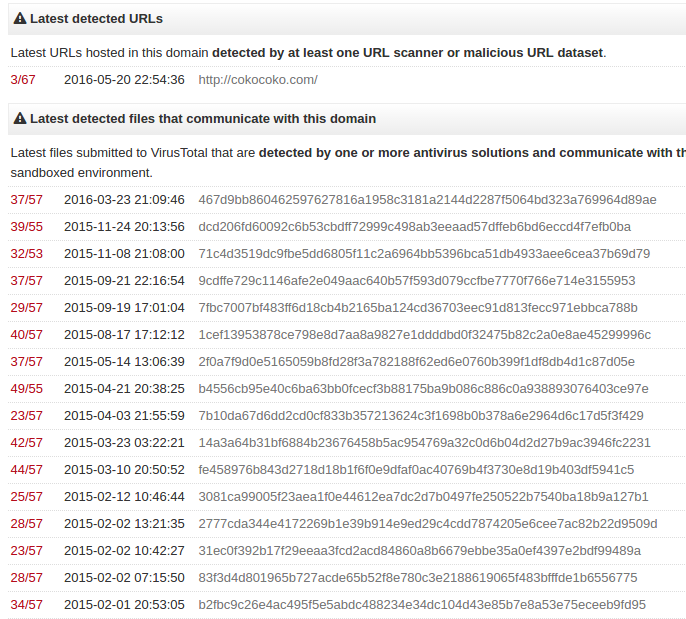
\includegraphics[scale=0.7]{vt-detect.png}
	\caption{Отчёт virustotal.com по домену cokocoko.com}
	\label{fig:vt}
\end{figure}

Как видно на рисунке~\ref{fig:vt}, этот домен действительно вредоносный. К нему обращалось множество модификаций вируса (это видно по SHA256 суммам от исполняемых файлов, которые взаимодействовали с этим доменом).

С помощью домена rwlfjbbqprgtgpfecascxcpblv.org было найдено приложение к отчету ФБР $\cite{fbi}$, связаному с наблюдением за ботнетом Zeus.

Что касается подхода с поиском сообществ, чаще всего встречаются тривиальные подграфы (две вершины и одно ребро), ощутимо реже встречаются более интересные конфигурации (<<звезды>> разных типов, деревья, подробно это описано в разделе~\ref{ssec:communitystruct}).
\begin{figure}[H]
	\centering
	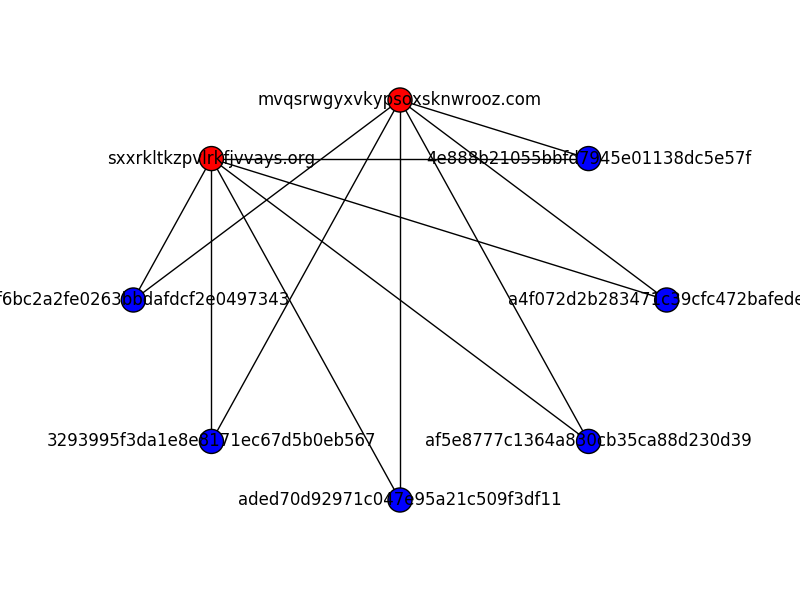
\includegraphics[scale=0.7]{mal-graph.png}
	\caption{Вредоносный подграф}
	\label{fig:mal-graph}
\end{figure}

На рисунке~\ref{fig:mal-graph} изображен один из <<интересных>> подграфов. Красным цветом отмечены вершины, соответствующие доменным именам, синим - hash+salt от ip адресов пользователей (по причине того, что недопустимо раскрывать реальные адреса пользователей). 

\section{Оценка работы классификатора для доменных имен}
Так как были использованы техники машинного обучения и построены классификаторы (построение описано в главе~\ref{chap:union-all}), стоит обратить внимание на формальные метрики оценки качества обученных классификаторов.

Естественно, все эти метрики вычисляются каждый раз во время процесса построения новых классификаторов и именно по ним принимается решение о выборе наилучшего экземпляра. За счет оценки по метрикам достигается автоматизация процесса обучения. Для демонстрации, я приведу небольшой пример ниже.

Возьмем случайный набор из 10 построенных классификаторов и выпишем значения основных метрик в таблицу~\ref{tab:metr}.

\begin{table}[H]
	\centering
	\caption{Значение формальных метрик для набора классификаторов}
	\label{tab:metr}
	\begin{tabular}{ |l|l|l|l|l|l|l|}
		\hline
		TP       & FP     & TN         & FN      & precision & recall & roc-auc \\ \hline
		874,0000 & 9.5000 & 15702.2500 & 38.5000 & 0.9893    & 0.9578 & 0.9929  \\ \hline
		798.0000 & 3.7500 & 7040.0000  & 27.7500 & 0.9953    & 0.9664 & 0.9962  \\ \hline
		849.5000 & 0.7500 & 14750.0000 & 29.5000 & 0.9991    & 0.9664 & 0.9943  \\ \hline
		887.7500 & 4.5000 & 14272.7500 & 26.2500 & 0.9950    & 0.9713 & 0.9936  \\ \hline
		861.5000 & 2.7500 & 14080.2500 & 43.7500 & 0.9968    & 0.9517 & 0.9914  \\ \hline
		847.5000 & 6.7500 & 17723.0000 & 41.2500 & 0.9921    & 0.9536 & 0.9937  \\ \hline
		544.0000 & 7.7500 & 6964.7500  & 41.5000 & 0.9860    & 0.9291 & 0.9953  \\ \hline
		949.2500 & 5.7500 & 20565.7500 & 45.5000 & 0.9940    & 0.9543 & 0.9924  \\ \hline
		797.2500 & 4.0000 & 15613.2500 & 34.5000 & 0.9950    & 0.9585 & 0.9919  \\ \hline
		968.5000 & 3.5000 & 14656.2500 & 30.7500 & 0.9964    & 0.9692 & 0.9932  \\ \hline
	\end{tabular}
\end{table}

Данные метрики подтверждают качество построенных классификаторов и, формально, говорят о пригодности использования описанного подхода в реальной жизни.

\chapter*{ЗАКЛЮЧЕНИЕ}
\addcontentsline{toc}{chapter}{ЗАКЛЮЧЕНИЕ}
В результате данной работы были изучены многочисленные статьи, произведен анализ их содержимого на предмет практической применимости. В сравнении с другими предложениями, текущее решение обладает важными качествами:
\begin{enumerate}
	\item Не требует труднодоступной информации (например данных pDNS и WHOIS).
	\item Не требует реверс-инжиниринга кода или запуска семплов вирусов в песочнице для анализа. Этот процесс всегда достаточно трудоемок и требует непосредственного участия высококвалифицированного специалиста.
	\item Процесс полностью автоматизирован и не требует вмешательства человека.
\end{enumerate}


<<В бою>>, эта техника показала себя хорошо, но в дальнейшем требуется больше внимания уделить <<охвату>> классификатора (минимизации ошибок 2 рода), чтобы находить больше вредоносных доменов а также автоматическому выбору порога по ROC кривой.

В данный момент, результат работы внедрен 	в компании SkyDNS и помогает предотвращать вредоносные коммуникации пользователей а также предупреждать их об опасности.

Задачи, поставленные во введении, достигнуты полностью. В результате анализа и работы был получен готовый программный продукт, который удовлетворяет требованиям бизнеса. 

В дальнейшем, планируется развивать направление, связанное с анализом структуры графа запросов:
\begin{enumerate}
	\item Cоздание инструмента, позволяющего в интерактивном режиме исследовать данный граф и искать в нем скрытые связи.
	\item Реализация автоматической классификация подграфов.
\end{enumerate}

\begin{thebibliography}{99}
	
	\addcontentsline{toc}{chapter}{СПИСОК ИСПОЛЬЗОВАННЫХ ИСТОЧНИКОВ}
			
	\bibitem{communication} Gunter Ollmann, ``Botnet Communication Topologies. Understanding the intricacies of botnet command-and-control'', 2009.
			
	\bibitem{groupact} Hyunsang Choi, Hanwoo Lee, Heejo Lee, Hyogon Kim, ``Botnet Detection by Monitoring Group Activities in
	DNS Traffic''.
			
	\bibitem{graphscore} Keisuke Ishibashi, Tsuyoshi Toyono, Makoto Iwamura, ``Botnet Detection Combining DNS and Honeypot Data''.
			
	\bibitem{rank} Frank Denis, ``Malware vs Big Data'', pp. 30 -- 31.
	\bibitem{commstruct} Y. Jin, E. Sharafuddin, and Z. L. Zhang, “Unveiling core network-wide communication patterns through application traffic activity graph decomposition,” in Proceedings of the eleventh international joint conference on Measurement and modeling of computer systems. ACM, 2009, pp. 49 -- 60.
	\bibitem{dnsrfc}  P. Mockapetris, ``DOMAIN NAMES - IMPLEMENTATION AND SPECIFICATION, RFC1035''.
	\bibitem{nmtf} C. Ding, T. Li, W. Peng, H. Park, ``Orthogonal nonnegative matrix t-factorizations for clustering'', in Proceedings of the 12th ACM SIGKDD
	international conference on Knowledge discovery and data mining, ser.
	KDD ’06. New York, NY, USA: ACM, 2006, pp. 126–135.
	\bibitem{bind} Jeroen Massar, ``DNSTAP: high speed DNS logging without packet capture'', pp. 29 -- 35.
	\bibitem{fbi} ``Appendix for FBI report about Zeus domains'', pp. 73, \url{https://www.justice.gov/opa/file/798036/download}.
\end{thebibliography}

\begin{appendices}
	\chapter{Скрипт для поиска вредоносных доменов}
	\label{appendix:code}
	\lstinputlisting[language=Python, breaklines=true, basicstyle=\footnotesize]{../suspicious-detection.py}
\end{appendices}


\end{document} 